\begin{wrapfigure}[0]{r}[0cm]{4cm}
	\vspace{-6cm}
  	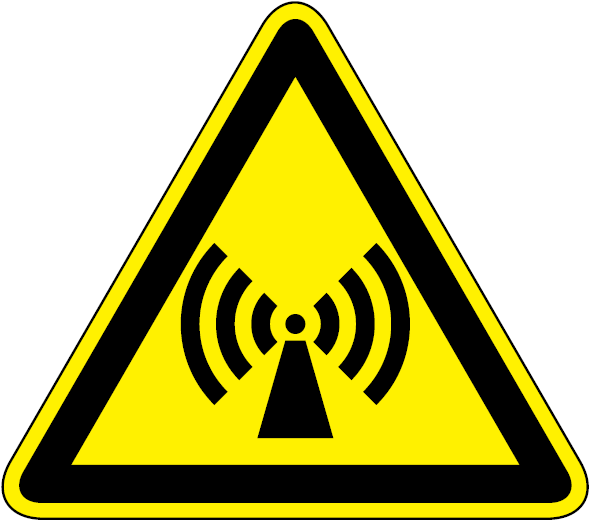
\includegraphics[scale=0.2]{EMV/Bilder/Symbol_Nichtionisierende_Strahlung}
  	\vspace{-6cm}
	\end{wrapfigure}

\section*{Theorie- und Prüfungsfragen}


\begin{enumerate} 
	\item \emph{\textbf{TK104}} Bei der Überprüfung des Ausgangssignals eines 75-Watt-Kurzwellen-Senders sollte die Dämpfung der Oberwellen in Bezug auf die Leistung der Betriebsfrequenz mindestens
	\begin{enumerate}
	\itemsep1pt\parskip0pt\parsep0pt
		\item[A] 20 dB betragen.
		\item[B] 40 dB betragen.
		\item[C] 60 dB betragen.
		\item[D] 100 dB betragen.
		\loesung{Lösung B}
		\end{enumerate} 
	\item \emph{\textbf{TK106}} In welchem Fall spricht man von Einstrahlungen bei EMV? Einstrahlungen liegen dann vor, wenn die HF ...
	\begin{enumerate}
	\itemsep1pt\parskip0pt\parsep0pt
		\item[A] über nicht genügend geschirmte Kabel zum gestörten Empfänger gelangt. 
		\item[B] über Leitungen oder Kabel in das gestörte Gerät gelangt.
		\item[C]   über das ungenügend abgeschirmte Gehäuse in die Elektronik gelangt.
		\item[D]  wegen eines schlechten Stehwellenverhältnisses wieder zum Sender zurück strahlt.
		\loesung{Lösung C}
		\end{enumerate}
	\item \emph{\textbf{TK107}} In welchem Fall spricht man von Störungen im Sinne von EMV? Störungen liegen dann vor, wenn ...
	\begin{enumerate}
	\itemsep1pt\parskip0pt\parsep0pt
		\item[A] unerwünschte Ausstrahlungen verursacht werden.
		\item[B] durch die hohe Feldstärke des Senders der Empfang auf anderen Frequenzen beeinflusst wird.
		\item[C]  durch den zu geringen Abstand zwischen einer Sende- und einer Empfangsantenne der Fernsehempfang durch einen Amateurfunksender gestört wird.
		\item[D]  ein Funkamateur mit seiner Sendefrequenz zu nah an den Rand des erlaubten Frequenzbereichs gelangt.
		\loesung{Lösung A}
		\end{enumerate}
	\item \emph{\textbf{TK103}} Welche sofortige Reaktion ist angebracht, wenn der Nachbar sich über HF-Störungen beklagt?
	\begin{enumerate}
	\itemsep1pt\parskip0pt\parsep0pt
		\item[A] Er sollte höflich darauf hingewiesen werden, dass es an seiner eigenen Einrichtung liegt.
		\item[B] Sie bieten höflich an, die erforderlichen Prüfungen in die Wege zu leiten.
		\item[C] Er sollte darauf hingewiesen werden, dass Sie hierfür nicht zuständig sind.
		\item[D] Sie benachrichtigen die Bundesnetzagentur.
		\loesung{Lösung B}
		\end{enumerate}
	\item \emph{\textbf{TK201}}  Wie kommen Geräusche aus den Lautsprechern einer abgeschalteten Stereoanlage möglicherweise zustande?
	\begin{enumerate}
	\itemsep1pt\parskip0pt\parsep0pt
		\item[A] Durch eine Übersteuerung des Tuners mit dem über die Antennenzuleitung aufgenommenen HF-Signal.
		\item[B] Durch Gleichrichtung starker HF-Signale in der NF-Endstufe der Stereoanlage.
		\item[C]  Durch Gleichrichtung der ins Stromnetz eingestrahlten HF-Signale an den Dioden des Netzteils.
		\item[D] Durch Gleichrichtung abgestrahlter HF-Signale an PN-Übergängen in der NF-Vorstufe.
		\loesung{Lösung B}
		\end{enumerate}
	\item \emph{\textbf{TK304}} Ein Funkamateur wohnt in einem Reihenhaus. An welcher Stelle sollte die KW-Drahtantenne angebracht werden, um störende Beeinflussungen auf ein Mindestmaß zu begrenzen?
	\begin{enumerate}
	\itemsep1pt\parskip0pt\parsep0pt
		\item[A] Rechtwinklig zur Häuserzeile mit abgewandter Strahlungsrichtung
		\item[B] Am gemeinsamen Schornstein neben der Fernsehantenne
		\item[C]  Entlang der Häuserzeile auf der Höhe der Dachrinne
		\item[D]  Möglichst innerhalb des Dachbereichs
		\loesung{Lösung A}
		\end{enumerate}	
	\item \emph{\textbf{TL213}}  Mit welcher Ausgangsleistung rechnen Sie im Fall des Personenschutzes, um den Sicherheitsabstand zu ermitteln?
	\begin{enumerate}
	\itemsep1pt\parskip0pt\parsep0pt
		\item[A] Mit der größten Ausgangsleistung des Transceivers zuzüglich Antennengewinns, korrigiert um den Gewichtungsfaktor für die verwendete Betriebsart.
		\item[B] Mit dem Mittelwert der Ausgangsleistung gemittelt über ein Intervall von 6 Minuten.
		\item[C]  Mit der durchschnittlich benutzten Ausgangsleistung gemittelt über den Betriebszeitraum und korrigiert um den Gewichtungsfaktor für die verwendete Betriebsart.
		\item[D]  Mit der maximalen Ausgangsleistung des verwendeten Senders zuzüglich 3 dB Messfehler.
		\loesung{Lösung B}
		\end{enumerate}	
	\item \emph{\textbf{TL211}} Sie möchten den Personenschutz-Sicherheitsabstand für die Antenne Ihrer Amateurfunkstelle für das 2-m-Band und die Betriebsart FM berechnen. Der Grenzwert im Fall des Personenschutzes beträgt 28 V/m. Sie betreiben eine Yagi-Antenne mit einem Gewinn von $11,5 dBd$. Die Antenne wird von einem Sender mit einer Leistung von $100 W$ über ein Koaxialkabel gespeist. Die Kabeldämpfung beträgt $1,5 dB$. Wie groß muss der Sicherheitsabstand sein?
	\begin{enumerate}
	\itemsep1pt\parskip0pt\parsep0pt
		\item[A] 6,18 m
		\item[B] 7,92 m
		\item[C] 2,50 m
		\item[D] 5,01 m
		\loesung{Lösung B}
		\end{enumerate}
	\item \emph{\textbf{TL302}} Welches Material und welcher Mindestquerschnitt ist bei einer Erdungsleitung zwischen einem Antennenstandrohr und einer Erdungsanlage nach DIN VDE 0855 Teil 300 für Funksender bis 1 kW zu verwenden?
	\begin{enumerate}
	\itemsep1pt\parskip0pt\parsep0pt
		\item[A] Ein- oder mehrdrähtiger - aber nicht feindrähtiger - isolierter oder blanker Kupferleiter mit mindestens $10 mm^2$ Querschnitt oder ein Aluminiumleiter mit mindestens $16 mm^2$ Querschnitt.
		\item[B] Ein- oder mehrdrähtiger - aber nicht feindrähtiger - isolierter oder blanker Kupferleiter mit mindestens $25 mm^2$ Querschnitt oder ein Aluminiumleiter mit mindestens $50 mm^2$ Querschnitt.
		\item[C]  Als geeigneter Erdungsleiter gilt ein Einzelmassivdraht mit einem Mindestquerschnitt von $16 mm^2$ Kupfer, isoliert oder blank, oder $25 mm^2$ Aluminium isoliert oder $50 mm^2$ Stahl.
		\item[D] Als geeigneter Erdungsleiter gilt ein Einzeldraht mit einem Mindestquerschnitt von $4 mm^2$ Kupfer, isoliert oder blank, oder $10 mm^2$ Aluminium isoliert.
		\loesung{Lösung C}
		\end{enumerate}
\end{enumerate}



